\chapter{Конструкторская часть}

В данном разделе представлены схемы алгоритмов сортировки и произведена оценка трудоемкости алгоритмов сортировки.

\section{Разработка алгоритма блочной сортировки}
На рис. \ref{img:block_sort_alg}~--~\ref{img:block_sort_alg_pos} представлена схема алгоритма блочной сортировки.

\begin{figure}[h!]
\centering
    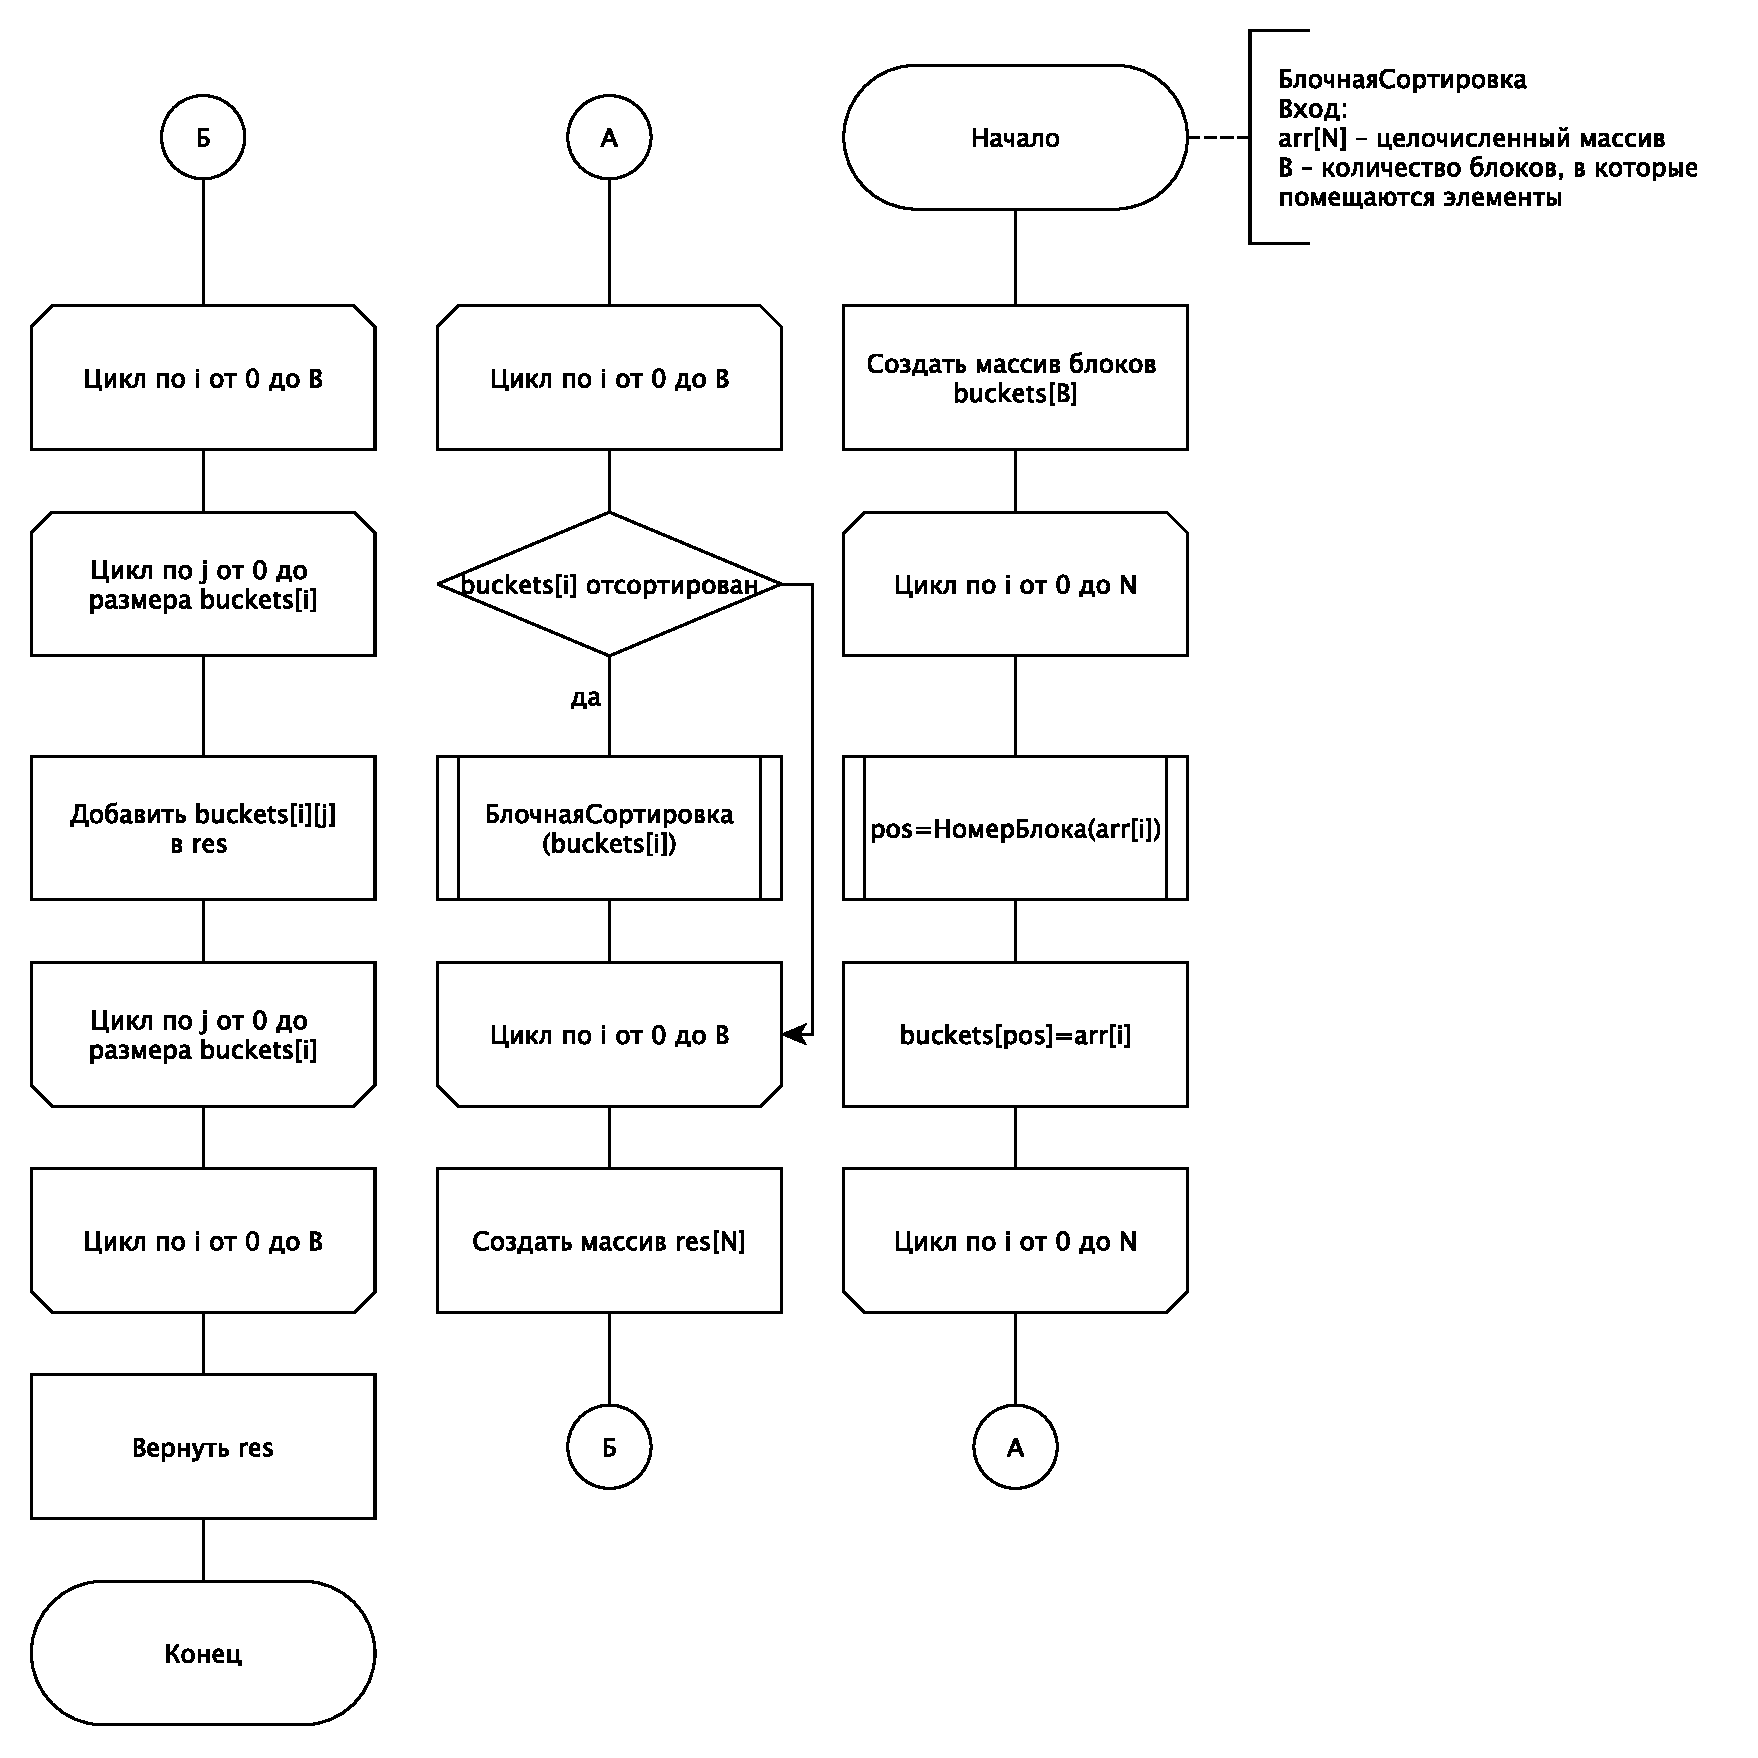
\includegraphics[width=0.9\linewidth]{block_sort_alg.pdf}
    \caption{Схема алгоритма блочной сортировки}
    \label{img:block_sort_alg}	
\end{figure}

\newpage

\begin{figure}[h!]
\centering
    \includegraphics[width=0.45\linewidth]{block_sort_alg_pos.pdf}
    \caption{Схема нахождения номера блока для элемента массива}
    \label{img:block_sort_alg_pos}	
\end{figure}

\newpage

\section{Разработка алгоритма пирамидальной сортировки}
На рис. \ref{img:heap_sort_alg}~--~\ref{img:heap_sort_alg_heapify} представлена схема алгоритма пирамидальной сортировки.

\begin{figure}[h!]
\centering
    \includegraphics[width=0.9\linewidth]{heap_sort_alg.pdf}
    \caption{Схема алгоритма пирамидальной сортировки}
    \label{img:heap_sort_alg}	
\end{figure}

\newpage

\begin{figure}[h!]
\centering
    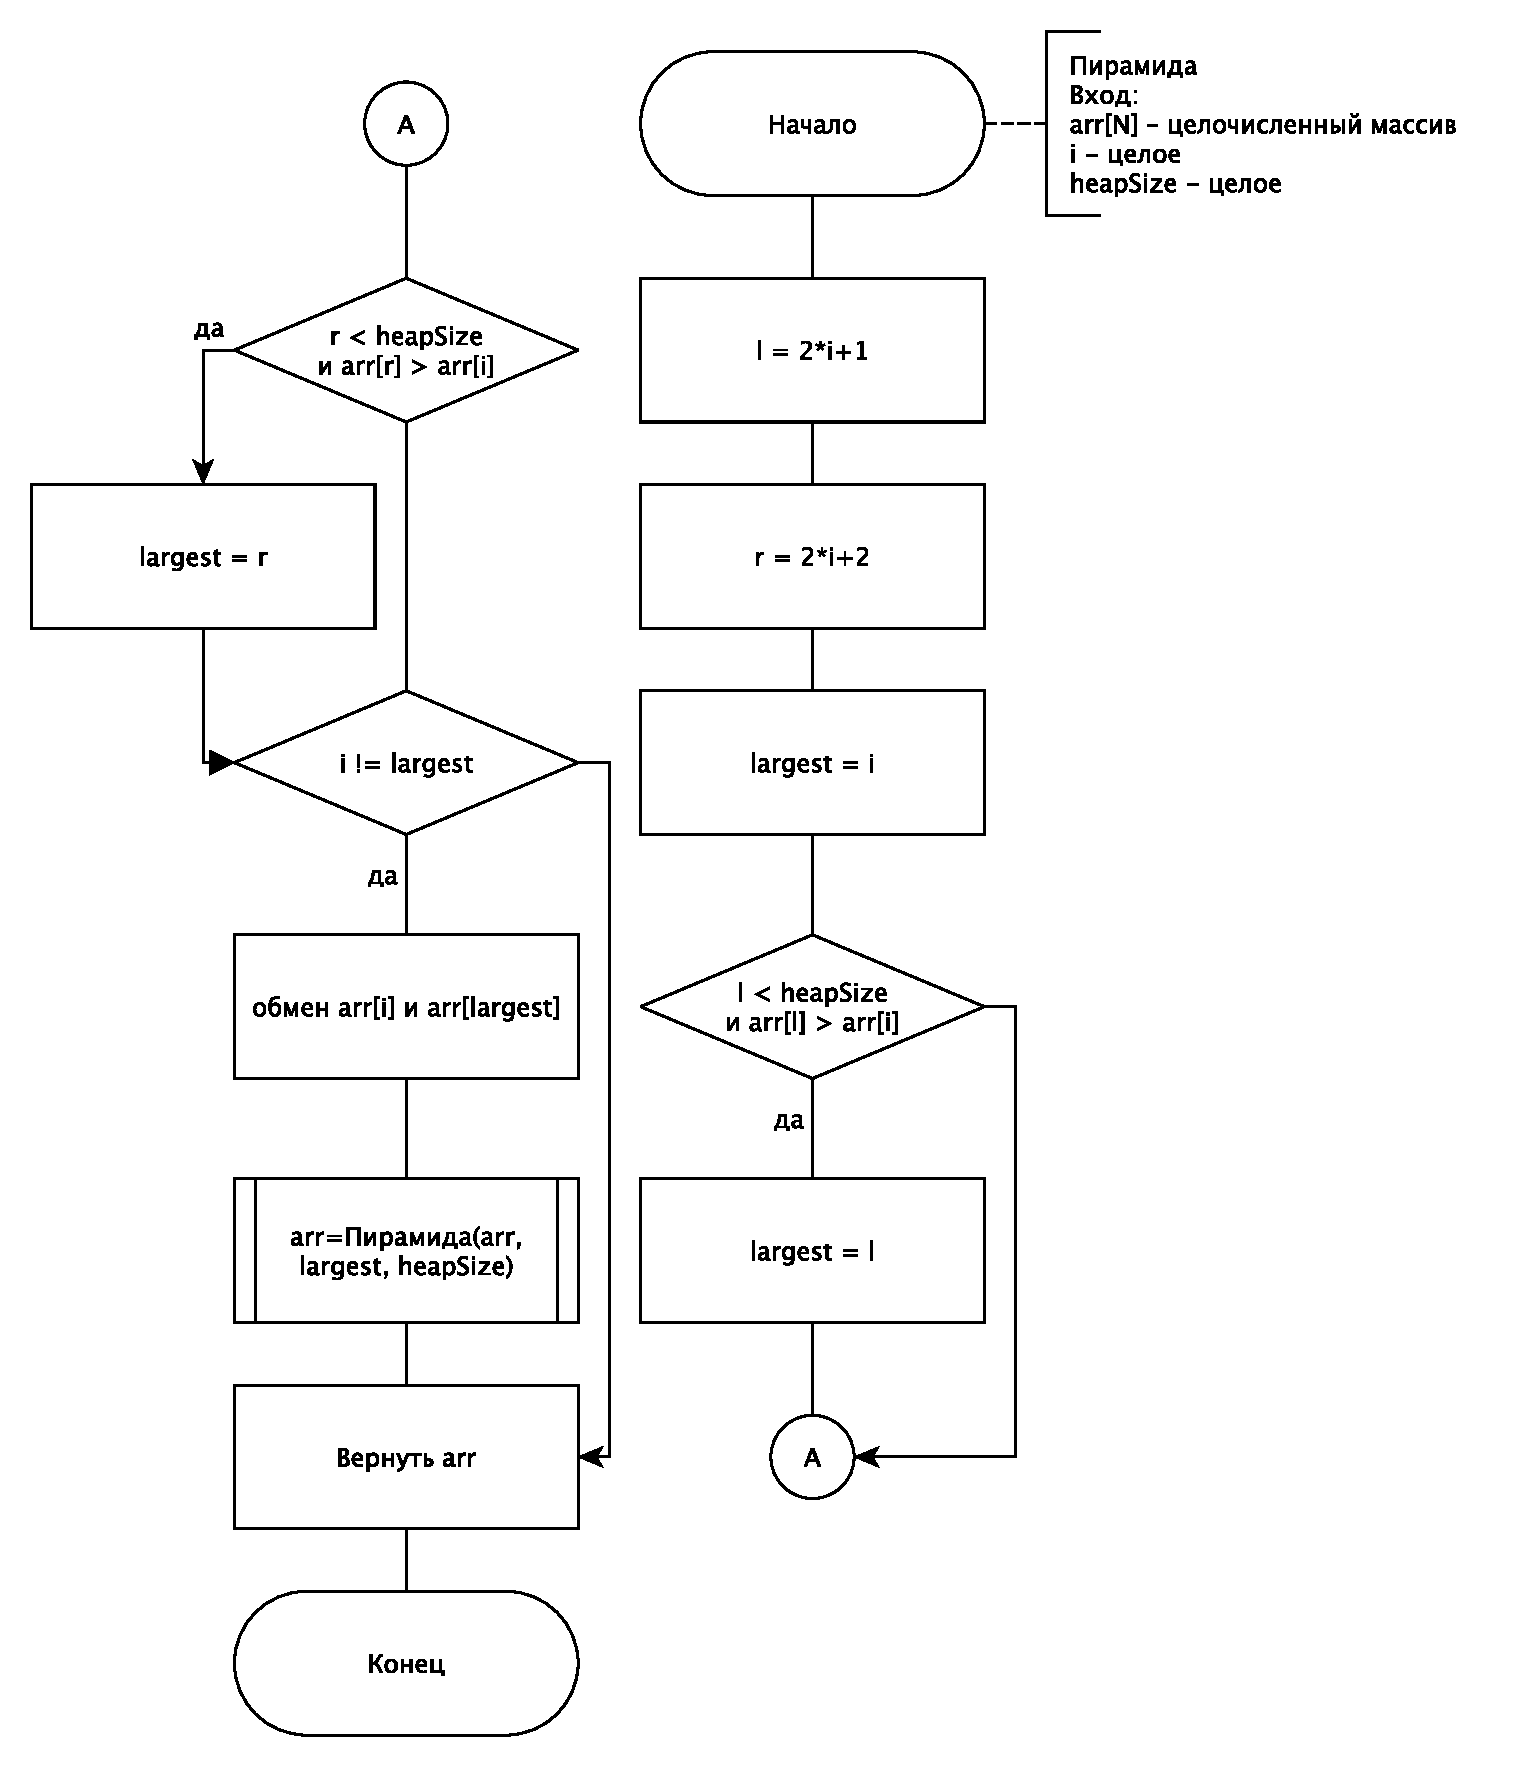
\includegraphics[width=0.9\linewidth]{heap_sort_alg_heapify.pdf}
    \caption{Схема алгоритма преобразование массива в пирамиду}
    \label{img:heap_sort_alg_heapify}	
\end{figure}

\newpage

\section{Разработка алгоритма сортировки подсчетом}
На рис. \ref{img:count_sort_alg} представлена схема алгоритма сортировки подсчетом.

\begin{figure}[h!]
\centering
    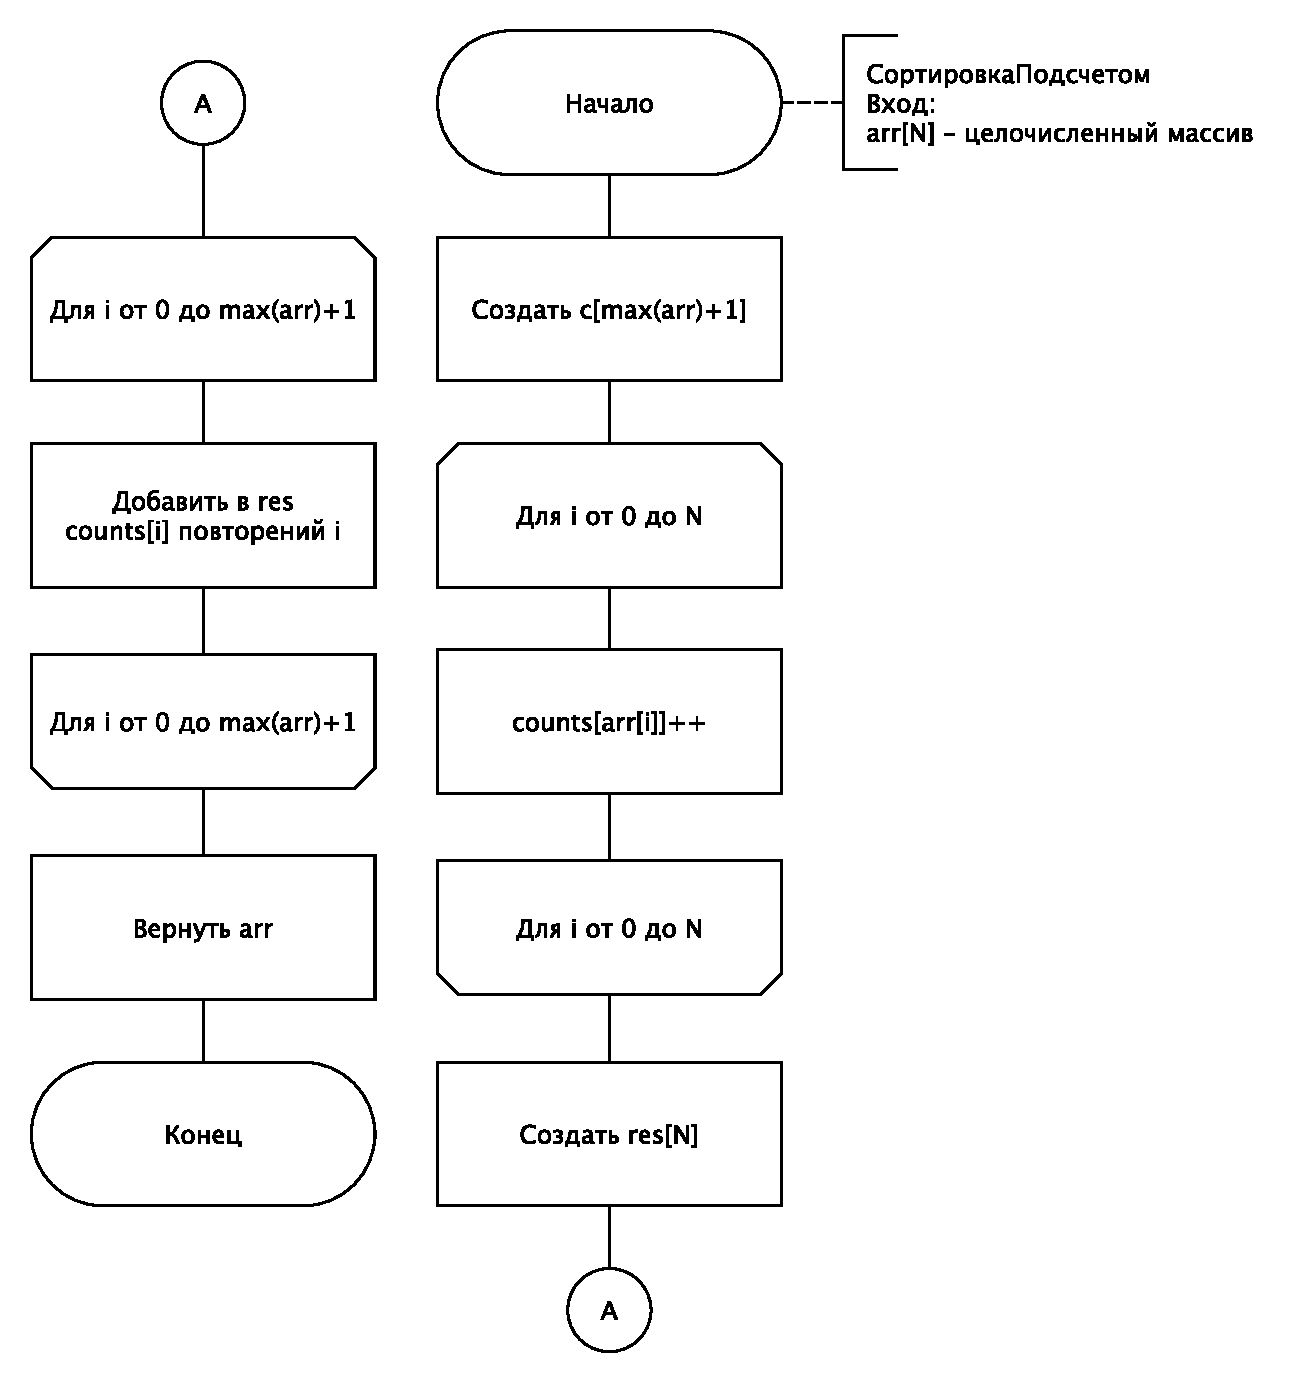
\includegraphics[width=0.7\linewidth]{count_sort_alg.pdf}
    \caption{Схема алгоритма сортировки подсчетом}
    \label{img:count_sort_alg}	
\end{figure}

\section{Оценка трудоемкости алгоритмов сортировки}

\subsection{Модель вычислений}
Для вычисления трудоемкости исследуемых алгоритмов необходимо ввести модель вычислений. 

Если обозначить трудоемкость некоторой операции $a$, как $f_a$, то можно ввести таблицу соответствия значения трудоемкости для базовых операций:


\begin{table}[h]
  \caption{\label{table:complexity} Таблица значений тредоемкости}
  \begin{center}
    \begin{tabular}{|l|r|}
      \hline
      Операция & Трудоемкость\\ \hline
      $:=$ & $1$ \\ \hline
      $+=$ & $1$ \\ \hline
      $-=$ & $1$ \\ \hline
      $+$ & $1$ \\ \hline
      $-$ & $1$ \\ \hline
      $<<$ & $1$ \\ \hline
      $>>$ & $1$ \\ \hline
      $[]$ & $1$ \\ \hline
      $++$ & $1$ \\ \hline
      $--$ & $1$ \\ \hline
      $>=$ & $1$ \\ \hline
      $<=$ & $1$ \\ \hline
      $==$ & $1$ \\ \hline
      $!=$ & $1$ \\ \hline
      $<$ & $1$ \\ \hline
      $>$ & $1$ \\ \hline
      $*$ & $2$ \\ \hline
      $/$ & $2$ \\ \hline
      $\%$ & $2$ \\ \hline
      вызов функции & $0$ \\ \hline
    \end{tabular}
  \end{center}
\end{table}

Трудоемкость условного блока можно ввести следующим образом:

\begin{equation}
	f_{if} = f_{cond} + \begin{cases}
		min(f_{in\_if}, f_{in\_else}) \quad \text{в лучшем случае}, \\
		max(f_{in\_if}, f_{in\_else}) \quad \text{в худшем случае},
	\end{cases}
\end{equation}

где

\begin{itemize}
	\item $f_{if}$~---~трудоемкость условного блока;
	\item $f_{cond}$~---~трудоемкость вычисления условия;
	\item $f_{in\_if}$~---~трудоемкость фрагмента после $if$;
	\item $f_{in\_else}$~---~трудоемкость фрагмента после $else$.
\end{itemize}

Трудоемкость цикла можно ввести следующим образом:


\begin{equation}
	f_{loop} = f_{init} + f_{cmp} + n \cdot (f_{body} + f_{cmp} + f_{inc}),
\end{equation}

где

\begin{itemize}
	\item $f_{loop}$~---~трудоемкость цикла;
	\item $f_{init}$~---~трудоемкость инициализирующего выражения;
	\item $f_{cmp}$~---~трудоемкость сравнения цикла;
	\item $f_{body}$~---~трудоемкость тела цикла;
	\item $f_{inc}$~---~трудоемкость инкремента.
\end{itemize}

\subsection{Трудоемкость алгоритма блочной сортировки}
Здесь и далее будут использоваться следующие обозначения:

\begin{itemize}
	\item $N$~---~количество элементов массива;
	\item $M$~---~максимальный элемент массива;
	\item $B$~---~количество элементов в одном блоке, известно, что
	\begin{equation}
		B \cdot M = N.
	\end{equation}
\end{itemize}

Трудоемкости нахождения максимума и минимума в массиве равны:

\begin{equation}
	f_{max} = 1 + 2 + 1 + 1 + N \cdot \left(1 + 1 + 2 + \begin{cases}
		1, & \text{если элемент больше максимума}, \\
		0, & \text{иначе},
	\end{cases}\right)
\end{equation}

\begin{equation}
	f_{max} = \begin{cases}
		5 + 5 \cdot N, & \text{в худшем случае}, \\
		5 + 4 \cdot N, & \text{в лучшем случае}.
	\end{cases} 
\end{equation}

\begin{equation}
	f_{min} = \begin{cases}
		5 + 5 \cdot N, & \text{в худшем случае}, \\
		5 + 4 \cdot N, & \text{в лучшем случае}.
	\end{cases} 
\end{equation}

Так как поиск максимальных и минимальных элементов отличаются только знаком сравнения элементов, причем эти знаки противоположны, то лучший случай для поиска максимума является худшим случаем для поиска минимума. 
Таким образом, можно полагать, что их суммарная трудоемкость будет равна

\begin{equation}
	f_{min, max} = 10 + 9 \cdot N.
\end{equation}


Трудоемкость расчета параметров для расчета размеров блока равна

\begin{equation}
	f_1 = f_{min, max} + 3 + 1 + 1 + 1 + 3 + 1 = 20 + 9 \cdot N.
\end{equation}

Трудоемкость размещения элементов по блокам равна

\begin{equation}
	f_2 = 2 + N \cdot (5 + 6 + 2) = 2 + N \cdot 13.
\end{equation}

Таким образом, трудоемкость блока с рекурсивным вызовом можно оценить, как

\begin{equation}
	f_3 = 2 + M \cdot \left(2 + 6 \cdot B\right) = 2 + 2 \cdot M + 6 \cdot N.
\end{equation}

Трудоемкость размещения отсортированных элементов из блоков в результирующий массив равна

\begin{equation}
	f_4 = 2 + M \cdot (2 + 2 + B \cdot (2 + 3)) = 2 + 4 \cdot M + 5 \cdot N.
\end{equation}

Трудоемкость одного вызова функции сортировки равна

\begin{equation}
	f_5 = f_1 + f_2 + f_3 + f_4,
\end{equation}

\begin{equation}
	f_5 = 26 + 33 \cdot N + 6 \cdot M,
\end{equation}

Для алгоритма блочной сортировки худшим случаем является тот, в котором в исходном массиве лежат отсортированные по убыванию слабо различающиеся элементы, которые в результате размещения будут расположены всего в двух блоках. Из-за проверки на отсортированность блоков, лучшим случаем будет являться отсортированный по возрастанию массив.

Так как функция сортировки будет содержать в себе рекурсивный вызов, то для расчета итоговой трудоемкости нужно умножить трудоемкость тела функции сортировки на глубину рекурсии. Глубина рекурсии в данном случае будет равна

\begin{equation}
	d = \begin{cases}
		1, & \text{в лучшем случае}, \\
		N, & \text{в худшем случае}.
	\end{cases}
\end{equation}

Таким образом, трудоемкость алгоритма блочной сортировки равна

\begin{equation}
	f = d \cdot f_5 = \begin{cases}
		33 \cdot N + 6 \cdot M + 26, & \text{в лучшем случае}, \\
		33 \cdot N^2 + 6 \cdot M \cdot N + 26 \cdot M, & \text{в худшем случае}.
	\end{cases}
\end{equation}

На основе вышеуказанных расчетов можно сделать вывод, что асимптотика алгоритма блочной сортировки равна $O(N)$ в лучшем случае, и $O(N^2)$ в худшем случае.

\subsection{Трудоемкость алгоритма пирамидальной сортировки}

Лучшим случаем для данного алгоритма можно назвать случай, когда все элементы массива равны.

Трудоемкость тела построения пирамиды равна

\begin{equation}
	f_{pyr body} = \begin{cases}
		6 + 1 + 5 + 1 + 5 + 1 + 8, & \text{в лучшем случае}, \\
		6 + 1 + 5 + 5, & \text{иначе}. \\
	\end{cases}
\end{equation}

\begin{equation}
	f_{pyr body} = \begin{cases}
		17, & \text{в лучшем случае}, \\
		27, & \text{иначе}. \\
	\end{cases}
\end{equation}

Так как в функции есть рекурсивный вызов, то ее трудоемкость следует считать, как трудоемкость тела функции, умноженную на глубину рекурсии. Глубина рекурсии будет равна

\begin{equation}
	d = \log_2 N.
\end{equation}

Таким образом, трудоемкость построения пирамиды будет равна

\begin{equation}
	f_{pyr} = d * f_{pyr body} = \begin{cases}
		17 \cdot \log_2 N, & \text{в лучшем случае}, \\
		27 \cdot \log_2 N, & \text{иначе}. \\
	\end{cases}
\end{equation}

Трудоемкость начального цикла построения пирамиды равна

\begin{equation}
	f_1 = 2 + \frac{N}{2} \cdot (2 + 1 + f_{pyr}),
\end{equation}

\begin{equation}
	f_1 = \begin{cases}
		2 + \frac{1}{2} \cdot 3 \cdot N + \frac{1}{2} \cdot 17 \cdot N \cdot \log_2 N, & \text{в лучшем случае}, \\
		2 + \frac{1}{2} \cdot 3 \cdot N + \frac{1}{2} \cdot 27 \cdot N \cdot \log_2 N, & \text{иначе}. \\
	\end{cases}
\end{equation}

Трудоемкость непосредственно цикла сортировки равна

\begin{equation}
	f_2 = 2 + N \cdot (7 + 1 + 2 + 1 + f_{pyr}),
\end{equation}

\begin{equation}
	f_2 = \begin{cases}
		2 + 11 \cdot N + 17 \cdot N \cdot \log_2 N, & \text{в лучшем случае}, \\
		2 + 11 \cdot N + 27 \cdot N \cdot \log_2 N, & \text{иначе}. \\
	\end{cases}
\end{equation}

Трудоемкость пирамидальной сортировки будет равна

\begin{equation}
	f = f_1 + f_2 = \begin{cases}
 	4 + 12,5 \cdot N + 25.5 \cdot N \cdot \log_2 N, & \text{в лучшем случае}, \\
 	4 + 12,5 \cdot N + 40.5 \cdot N \cdot \log_2 N, & \text{иначе}.
 \end{cases}
\end{equation}

Таким образом, асимптотика алгоритма пирамидальной сортировки равна $O(N \cdot \log N)$.

\subsection{Трудоемкость алгоритма сортировки подсчетом}

Трудоемкость заполнения вспомогательного массива равна

\begin{equation}
	f_1 = 2 + 4 \cdot N.
\end{equation}

Трудоемкость размещения элементов в результирующий массив равна

\begin{equation}
	f_2 = 2 + R \cdot (2 + Q \cdot (2 + 3)),
\end{equation}

где $R$~---~максимальное число в массиве, $Q$~---~количество элементов, равных данному числу.

\begin{equation}
	f_2 = 2 + 2 \cdot R + 5 \cdot Q \cdot R = 2 + 2 \cdot R + 5 \cdot N.
\end{equation}

Трудоемкость алгоритма сортировки подсчетом будет равна

\begin{equation}
	f = f_1 + f_2 = 4 + 9 \cdot N + 2 \cdot R.
\end{equation}

В данном случае расположение элементов не влияет на скорость алгоритма, влияет только величина элеменов. Таким образом, худшим случаем для данного алгоритма будет сортировки больших чисел. Лучшим случаем будет сортировка одинаковых элементов небольшого размера, например, сортировка нулей. Асимптотика данного алгоритма равна $O(N + R)$.

\newpage